%!TEX root = curso_EDA_SLIDES.tex

%\title{Estrutura de Dados \\ Estrutura de dados Linear: Lista} 

\section{Listas}

\begin{frame}
\begin{center}
{\Large Capítulo xxxxx -- Listas}

Pontos fundamentais a serem cobertos:

\begin{enumerate}
  \item 
  \item 
  \item 
\end{enumerate}

\end{center}

\end{frame}
%--------------------



\section{Lista Lineares Estáticas}
  \begin{frame}{Introdução}    
		\begin{itemize}
			\item Uma seqüência de nós ou elementos dispostos em uma ordem estritamente linear.
			\item Cada elemento da lista é acessível um após o outro, em ordem.
			\item Pode ser implementada de várias maneiras			
				\begin{enumerate}
					\item Em um vetor
					\item Em uma estrutura que tem um vetor de tamanho fixo e uma variável para armazenar o tamanho da lista.
				\end{enumerate}
		\end{itemize}
  \end{frame}
  
\begin{frame}{Definição}
     \begin{block}{Definição}
       Um conjunto de nós, $x_1, x_2, x_3, \cdots, x_n$, organizados estruturalmente de forma a refletir as posições relativas dos mesmos. Se $n > 0$, então $x_1$ é o primeiro nó. \\
       Seja $L$ uma lista de $n$ nós, e $x_k$ um nó $\in$ L e $k$ a posição do nó em $L$. Então, $x_k$ é precedido pelo nó $x_{k-1}$ e seguido pelo nó $x_{k+1}$. O último nó de $L$ é $x_{n-1}$. Quando $n = 0$, dizemos que a lista está vazia.
     \end{block}     
\end{frame}

\begin{frame}{Representação}
\begin{itemize}
	\item Os nós de uma lista são armazenados em endereços contínuos.
	\item A relação de ordem é representada pelo fato de que se o endereço do nó $x_i$ é conhecido, então o endereço do nó $x_{i+1}$ também pode ser determinado. 	
	\item A Figura \ref{fig:lista-linear-repre} apresenta a representação de uma lista linear de $n$ nós, com endereços representados por $k$
\end{itemize}
\begin{figure}[ht]
	\centering
		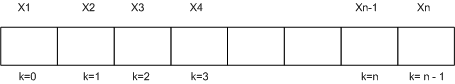
\includegraphics[width=.6\textwidth]{figs/fig_listas/lista-linear.png}				\caption{Exemplo de representação de lista.}	
				\label{fig:lista-linear-repre}
			\end{figure} 
\end{frame}

\begin{frame}[fragile,c]{Representação}
\begin{itemize}
	\item Para exemplificar a implementação em C, vamos considerar que o conteúdo armazenado na lista é do tipo inteiro.
	\item A estrutura da lista possui a seguinte representação:	
\end{itemize}
\begin{lstlisting}[language=C]
  struct lista{
    int cursor;
    int elemento[N];
  }
  typedef struct lista Lista;
\end{lstlisting}
\begin{itemize}
	\item Trata-se de uma estrutura heterogênea constituída de membros distintos entre si. Os membros são as variáveis \alert{\textit{cursor}}, que serve para armazenar a quantidade de elementos da lista e o vetor \alert{\textit{elemento}} de inteiros que armazena os nós da lista.
\end{itemize}
\end{frame}

\begin{frame}[fragile,c]{Representação}
\begin{itemize}
	\item Para atribuirmos um valor a algum membro da lista devemos utilizar a seguinte notação:

\small	
\begin{lstlisting}[language=C]
Lista->elemento[0] = 1 - atribui o valor 1 ao primeiro elemento da lista.
Lista->elemento[n-1] = 4 - atribui o valor 4 ao ultimo elemento da lista.
\end{lstlisting}
\end{itemize}
\end{frame}  

\begin{frame}{Operações Primitivas}
  \begin{itemize}
	  \item As operações básicas que devem ser implementadas em uma estrutura do tipo Lista são:		
  \end{itemize}
  \begin{table}[!htpb]
			  \centering
						\begin{tabular}{l|l}
						    \hline \textbf{Operação} & \textbf{Descrição} \\
						    \hline criar() & cria uma lista vazia.\\
						    \hline inserir(l,e) & insere o elemento \textit{e} no final da lista \textit{l}.\\
						    \hline remover(l,e) & remove o elemento \textit{e} da lista \textit{l}.\\
						    \hline imprimir(l) & imprime os elementos da lista \textit{l}.\\
						    \hline pesquisar(l,e) & pesquisa o elemento \textit{e} na lista \textit{l}.\\
						    \hline 
						\end{tabular}
						\caption{Operações básicas da estrutura de dados lista.}
				\end{table}
\end{frame}
 
\begin{frame}{Operações auxiliares}   
			\begin{itemize}
				\item Além das operações básicas, temos as operações ``auxiliares''. São elas:
			\end{itemize}
			\begin{table}[!htpb]
			  \centering
						\begin{tabular}{l|l}
						    \hline \textbf{Operação} & \textbf{Descrição} \\						    
						    \hline empty(l) & determina se a lista \textit{l} está ou não vazia.\\
						    \hline destroy(l) & libera o espaço ocupado na memória pela lista \textit{l}.\\
						    \hline 
						\end{tabular}
						\caption{Operações auxiliares da estrutura de dados lista.}
				\end{table}
  \end{frame}


\begin{frame}[fragile,plain]{Interface do Tipo Lista}
\footnotesize
\begin{lstlisting}[language=C]
/* Aloca dinamicamente a estrutura lista, inicializando 
 * seus campos e retorna seu ponteiro. A lista depois 
 * de criada terah tamanho igual a zero.*/
Lista* criar(void);

/* Insere o elemento e no final da lista l, desde que,
 * a lista nao esteja cheia.*/
void inserir(Lista* l, int e);

/* Remove o elemento e da lista l,
 * desde que a lista nao esteja vazia e o elemento
 * e esteja na lista. A funcao retorna 0 se o elemento 
 * nao for encontrado na lista ou 1 caso contrario. */
void remover(Lista* l, int e);

/* Pesquisa na lista l o elemento e. A funcao retorna 
 * o endereco(indice) do elemento se ele pertencer a lista
 * ou -1 caso contrario.*/
int pesquisar(Lista* l, int e);

/* Apresenta os elementos da lista l. */
void imprimir(Lista* l);
\end{lstlisting}
\end{frame}

\begin{frame}{Implementação da Lista}
\begin{itemize}
	\item A utilização de vetores para implementar a lista traz algumas vantagens como:	
		\begin{enumerate}
			\item Os elementos são armazenados em posições contíguas da memória;
			\item Economia de memória, pois os ponteiros para o próximo elemento da lista são explícitos.
		\end{enumerate}
		\item No entanto, as desvantagens são:		
			\begin{enumerate}
				\item Custo de inserir/remover elementos da lista;
				\item Limitação da quantidade de elementos da lista.
			\end{enumerate}
\end{itemize}
\end{frame}

\begin{frame}[fragile,c]{Função de Criação}
	\begin{itemize}
		\item A função que cria uma lista, deve criar e retornar uma lista vazia;
		\item A função deve atribuir o valor zero ao tamanho da lista, ou seja, fazer $l->cursor = 0$, como podemos ver no código abaixo.
		\item A complexidade de tempo para criar a lista é constante, ou seja, $O(1)$.
	\end{itemize}
\begin{lstlisting}[language=C]
/*
 * Aloca dinamicamente a estrutura lista, inicializando seus
 * campos e retorna seu ponteiro. A lista depois de criada
 * terah tamanho igual a zero.
 */
Lista* criar(void){
  Lista* l = (Lista*) malloc(sizeof(Lista));
  l->cursor = 0;
  return l;
}
\end{lstlisting}
\end{frame}

\begin{frame}[fragile,c]{Função de Inserção}  
	\begin{itemize}
		\item A inserção de qualquer elemento ocorre no final da lista, desde que a lista não esteja cheia.
		\item Com isso, para inserir um elemento basta atribuirmos o valor ao elemento cujo índice é o valor referenciado pelo campo \textit{cursor}, e incrementar o valor do cursor, ou seja fazer $l->elemento[l->cursor++] = valor$, como podemos verificar no código abaixo, a uma complexidade de tempo constante, $O(1)$.
	\end{itemize}

\footnotesize
\begin{lstlisting}[language=C]
/*
 * Insere o elemento e no final da lista l, desde que,
 * a lista nao esteja cheia.
 */
void inserir(Lista* l, int e){
  if (l == NULL || l->cursor == N){
    printf("Error. A lista esta cheia\n");
  }else{
    l->elemento[l->cursor++] = e;
  }
}
\end{lstlisting}	
\end{frame}

\begin{frame}[fragile,c]{Função de Remoção} 
	\begin{itemize}
		\item Para remover um elemento da lista, primeiro precisamos verificar se ele está na lista, para assim removê-lo, e deslocar os seus sucessores, quando o elemento removido não for o último.
		\item A complexidade de tempo da função de remoção é $O(n)$, pois é necessário movimentar os $n$ elementos para remover um elemento e ajustar a lista.
	\end{itemize}
	
\footnotesize
\begin{lstlisting}[language=C]
/* remove um elemento da lista */
void remover(Lista* l, int e){     
  int i, d = pesquisar(l,e);
  if (d != -1){
    for(i = d; i < l->cursor; i++)
    {
      l->elemento[i] = l->elemento[i + 1];
    }
    l->cursor--;
  }  
}
\end{lstlisting}	
\end{frame} 

\begin{frame}[fragile]{Função de Pesquisa} 
	\begin{itemize}
		\item Para pesquisar um elemento qualquer na lista é necessário compará-lo com os elementos existentes, utilizando alguns dos algoritmos de busca conhecidos;
		\item A complexidade de tempo dessa função depende do algoritmo de busca implementado. Se utilizarmos a busca seqüencial, a complexidade da função será $O(n)$. No entanto, é possível baixá-lo para $O(n\log n)$.
	\end{itemize}

\footnotesize
\begin{lstlisting}[language=C]
int pesquisar(Lista* l, int e){
  if (l == NULL)
    return;
  
  int i = 0;
  while (i <= l->cursor && l->elemento[i] != e)
    i++;
        
  return i > l->cursor ? -1 : i;
}
\end{lstlisting}
\end{frame}

\begin{frame}[fragile]{Função de Impressão}
\begin{itemize}
		\item A impressão da lista ocorre através da apresentação de todos os elementos compreendidos entre o intervalo: $[0.. l->cursor]$.
		\item A complexidade de tempo da função de impressão é $O(n)$, pois no pior caso, quando lista estiver cheia, é necessário percorrer os $n$ elementos da lista.
	\end{itemize}
	
\begin{lstlisting}[language=C]
/*Apresenta os elementos da lista l. */
void imprimir(Lista* l){
 int i;
 for(i = 0; i < l->cursor; i++)
   printf("%d ", l->elemento[i]);
 printf("\n");  
}
\end{lstlisting}	
\end{frame}

\begin{frame}[fragile,c]{Exemplo de Uso da Lista}
\footnotesize
\begin{lstlisting}[language=C]
#include <stdio.h>
#include "list.h"

int main(void)
{
    Lista* l = criar();
    int i, j = 4;
    
    /* Inseri 5 elementos na lista */
    for (i = 0; i < 5; i++)
      inserir(l,j * i);
    
    /* Apresenta os elementos inseridos na lista*/    
    imprimir(l);
    /* Remove o segundo elemento da lista*/
    remover(l,j);
    /* Apresenta os elementos da lista */    
    imprimir(l);        
}
\end{lstlisting}
\end{frame} 


\begin{frame}{Referências}
	\begin{enumerate}
		\item Tenenbaum, A. M., Langsam, Y., and Augestein, M. J. (1995). Estruturas de Dados Usando C. MAKRON Books, pp. 207-250.
		\item Wirth, N. (1989). Algoritmos e Estrutura de dados. LTC, pp. 151-165.
	\end{enumerate}
\end{frame}
